\documentclass{article}

\usepackage[english]{babel}
\usepackage[a4paper,top=2cm,bottom=2cm,left=3cm,right=3cm,marginparwidth=1.75cm]{geometry}
\usepackage{amsmath}
\usepackage{graphicx}
\usepackage[colorlinks=true, allcolors=blue]{hyperref}

\title{Exploring and Predicting Heart Disease Trends: An IR System Using  Health Indicators}
\author{Fabian Baischer, Patrick Berchtold, Alexander Niederreiter, Raphael Hutten}

\begin{document}
\maketitle


\section{Abstract}

This project focuses on building a tool to predict a person’s risk of heart diseases based on their health information, and recommend drugs in case of risk.
We are using a dataset from Kaggle called "Indicators of Heart Disease",
which includes health details like BMI, smoking status, physical activity, and other personal information, to predict the heart disease risk,
and another dataset called "Drug Dataset: Uses, Side Effects and User Reviews" to recommend drugs.
Our goal is to train a machine learning model to estimate the likelihood of heart disease,
whose output we use to retrieve drug information to recommend medication.\\
The user will input their health details into a web frontend, which is then fed into our prediction model, which calculates a risk score for heart disease.\\
Overall, this project combines machine learning for medical predictions with information retrieval for drug recommendations,
so people can easily check their heart health and take action.
We aim to create a simple and accessible tool to help with early detection and prevention of heart disease.


\section{Main task}
The main question that our work is trying to solve:\\
We plan to build a complete system, using multiple techniques of machine learning and information retrieval. Moreover, to guarantee a good user experience, 
we create a website where the user can enter all the necessary health information. The front-end will be a vue app and the back-end will be a Flask server.
Based on this user input, he will then get a ranking of the best fitting medicals to this query.
To be more specific, this is the flow chart description that we have in mind:
\begin{itemize}
    \item The user enters his health data. The HTML form will include all the features from the heart disease dataset which is described in the latter section.
    \item After that the Python Flask server will load the previously generated heart disease ai model and predict whether the user is of a risk to a heart disease or not.
    \item If the user is at risk for heart disease, we then use the second dataset which includes medicine data.
    \item With the features from the user input, we rank the best fitting medicine for the user.
    \item The server then sends the top 5 best fitting medicals back to the frontend.
    \item On top of the names, we will further display all the additional data for each of the five entries in the drug dataset. This includes pictures of the drugs, possible side effects, etc.
\end{itemize} 

% The datasets that we want to use is originally from \textbf{CDC - U.S. Centers for disease control and prevention}. This organization has set up a survey system which started in 1984.
%  The so called \textbf{BRFSS - Behavioral Risk Factor Surveillance System} is a survey on American citizens which conducts questions about health-related risk behaviors, 
%  chronic health conditions and use of preventive services. By now, the BRFSS collects a yearly data from more than 400,000 adults. With that it is the largest conducted health survey 
%  system in the world.\\
% On Kaggle, the dataset from the year 2020 is available. The goal is to fit the most accurate model on this dataset to predict efficiently how likely it is for an adult to gain a heart 
% disease. However, the original data contains nearly 300 variables which was reduced to the most important 40 variables by the author who published this set on Kaggle. Moreover, 
% there exist two different versions of the dataset. With NaNs and without NaNs in it. We will decide which version we want to build on, once we have a clearer structure in which way
% we want to design our model. Furthermore, the careful decision if and with what we want to substitute the NaNs.\\


   


\section{Visual Depiction}
\begin{center} 
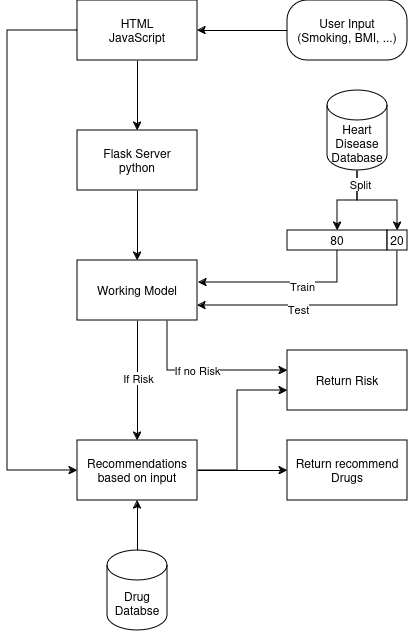
\includegraphics[scale=.75]{Hearth_death.drawio(1).png}
\end{center}
As you can see in the graphic above, we have the user write an input. Of course we give them some hints before that, what they should to talk about in their input. We process that using the ChatGPT API to get data in a comprehensible way for our trained model.
\\
The model we train ourselves beforehand, splitting our dataset 80/20 for training and evaluation until we are satisfied with the current state.
\\
We use the data we get back and the ChatGPT API again to write a text, which can give the User a detailed explanation about our calculated probability and the reasoning for it.

\newpage

\section{Dataset + Processing}

% resources used
\subsection{Indicators of Heart Disease}
We use the dataset "Indicators of Heart Disease" found on Kaggle\footnote{https://www.kaggle.com/datasets/kamilpytlak/personal-key-indicators-of-heart-disease},
which contains 3 tables: a dataset from 2020 (which we will not use),
and two updated versions from 2022.
One of the 2022 tables is simply a subset of the other table where every row which is missing data in any column has been removed.
The complete one is called \texttt{heart\_2022\_with\_nans}, containing $445,132$ rows,
and the stripped one is called \texttt{heart\_2022\_no\_nans}, containing $246,022$.
Depending on our needs, we will use one of the newer tables:
If \texttt{heart\_2022\_no\_nans} contains enough rows to build a proper model,
we will use it, since that way we don't need special handling for NaN rows.
Since one is just a subset of the other, the columns are the same in both tables.
Most of the tables are about the patient's health, so they will be included in our model:

\begin{itemize}
    \item \textit{Sex} $\in$ \{Male, Female\}
    \item \textit{GeneralHealth} $\in$ \{Poor, Fair, Good, Very Good, Excellent\}
    \item \textit{PhysicalHealthDays} $\in\ \{ 0,\ \dots,\ 30 \}$\\
    $60\%$ of the rows have a value of $0$ here, so we will instead map this to
    \{None, Low, High\}, where $0 = $ None, $<15 = $ Low, and $\geq15 =$ High.
    \item \textit{MentalHealthDays}  $\in\ \{ 0,\ \dots,\ 30 \}$\\
    The same rules as for \textit{PhysicalHealthDays} apply here.
    \item \textit{LastCheckupTime} $\in\ \{<1\ \text{year},\ <2\ \text{years},\ <5\ \text{years},\ \geq 5\ \text{years}\}$
    \item \textit{PhysicalActivities} $\in$ \{True, False\}
    \item \textit{SleepHours}  $\in\ \{ 1,\ \dots,\ 24 \}$\\
    There are rows with $24$ here, which we do not view as realistic.
    We will simply drop rows with $>16$.
    \item \textit{RemovedTeeth} $\in$ \{None, 1 to 5, 6+, All\}
    \item \textit{HadHeartAttack} $\in$ \{True, False\}
\end{itemize}

The last column is \textit{State}, which is either one of 5 US states,
which also hints at the sample population of this study.
We do not expect this column to have a major impact on heart attacks,
and since this is only limited to a small number of US states, we do not include it in our model.



\subsection{Drug Dataset: Uses, Side Effects and User Reviews}
For the drug recommendations we use the dataset "Drug Dataset: Uses, Side Effects and User Reviews", which is also found on Kaggle\footnote{https://www.kaggle.com/datasets/aadyasingh55/drug-dataset}. It has over 11496 medications with different columns representing different factors we need for the recommendation. Those consist of:

\begin{itemize}
    \item \textit{Medicine Name} contains the string
    \item \textit{Composition} contains the main ingredient which we need for transparency
    \item \textit{Uses} is necessary for our evaluation
    \item \textit{Side effects} is also necessary for our evaluation
    \item \textit{Image URL} is necessary for the feedback to the user, since buying the wrong medicine due to confusing names could be an issue
    \item \textit{Manufacturer} not necessary
    \item \textit{Excellent Review} necessary for evaluation
    \item \textit{Average Review} necessary for evaluation
    \item \textit{Poor Review} necessary for evaluation
\end{itemize}


\section{Methods/Models}
After successfully pre-processing and cleaning the dataset from Kaggle, we can now begin by selecting relevant features from the dataset, corresponding to the input made by the user. Since we do not force people to give us their data about their health, we need to find out what we were given and also if it is useable for our database. It has to be noted, that not all the factors presented in the dataset have the same impact on heart disease risk. This means that a fitting weighting scheme has to be applied to the different factors (e.g. importance scores). Once our features are selected and prepared, we experiment with several machine learning models to identify the one that provides the best predictive accuracy. Some of our candidate models include methods like linear regression (if we want to give a risk score), logistic regression (if we want specific risk groups), decision trees, random forest and Gradient Descent/Boosting. These models are selected for their ability to handle both categorical and numerical data efficiently and provide accurate predictions of heart disease risk. If we decide to use the classification approach (different risk classes), some important metrics to decide, how well these models perform are for example accuracy (overall correctness of the model), precision (positive predictions that are actually correct) and recall (actual positives that were correctly identified). We then want to utilize a cross-validation method (e.g. k-fold cross-validation) to evaluate the performance of machine learning models and ensuring that they respond correct to unseen data. Using cross-validation can help us assess the effectiveness of our models when predicting heart disease risk based on user inputs. If the model decides, that the user is at a high risk of getting a heart disease we will start process the user input correctly for our drug database so we can use it for a more accurate recommendation for the specific patient. There is no drug "for smoker", but different drugs could resolve into a lower blood oxygen or iron levels, which could be a risk for smokers. This has to be accounted for. Therefore we search for different words and definitions described in the side effects, but also benefits using a cosine similarity. If we have found the 5 best recommendations for this specific user, we return the recommendation to the user. 

\newpage


\section{Evaluation}

For the evaluation, it will be a strong interchange with the model building and fitting. After training a model, we have to test it and also measure the performance. For this, we need to select appropriate evaluation metrics. Moreover, it could be the case that the heart disease dataset it strongly imbalanced, meaning that one class (e.g. \textbf{no} heart disease) is much more frequent than other (e.g. heart disease). To deal with this, we must also consider to have a look into metrics like the precision-recall curve or the ROC curve.\\
Another design choice that must be made is, whether we use a binary indicator or a float score, to measure the likeliness of a heart disease. Using a float score would result in more precision, however some evaluation metrics are more suitable for binary classification then others.

\section{Group number, members and tentative roles}

We are group number 4, consisting of the following members:
\begin{itemize}
    \item Fabian Baischer
    \item Patrick Berchtold
    \item Alexander Niederreiter
    \item Raphael Hutten
\end{itemize}
Fabian Baischer will be responsible for setting up the server and the UI on the website. That means getting a server for the model, hosting it, and let it communicate with a repository so we can push code and change the model accordingly when it comes to any mistakes.
\vspace{1em}
Patrick Berchtold is tasked with setting up the model and validate the database so it can give an accurate decision. He will also need to preprocess the input made by the user accordingly because smoking a little and smoking a lot makes a big difference. This is a very important task which comes with a lot of decisions since the following things have to be taken into consideration:
\begin{itemize}
    \item It must be carefully evicted which model. 
    \item The model should neither underfit nor overfit but aim for the perfect balance between simplicity and accuracy.
    \item How to deal with missing values.
    \item What approach would be the best for categorical variables.
    \item Test if cross validation leads to better results.
    \item Using pipelines to fit multiple models and filter out the best ones.
    \item Maybe even use Gradient Boosting with multiple cycles to get a state-of-the-art highly accurate model.
\end{itemize}
\vspace{1em}
Alexander Niederreiter and Raphael Hutten will concentrate on the recommended drug system based on the User Input. For that they will also need to preprocess the data accordingly, since the database doesn't just say "heart disease", but has different kind of diseases, side effects and uses. To accurately represent the conditions and asked questions for the model and also use the input for different descriptions made by different companies without overseeing working drugs due to synonyms used in the descriptions. (eg. Heart disease, Cardiac disease).

\end{document}
